\subsubsection{TPLAN-RAIZ}

\textbf{TPLAN-RAIZ (TIPO-DE-PLANTA-RAIZ):} Essa variável está associada à profundidade do sistema radicular da planta no solo, ou, à Profundidade Efetiva das raízes da planta onde se concentram 80\% de suas raízes. Quanto maior a profundidade das raízes, maior a
necessidade de dotação hídrica.

\begin{table}[h!]
	\centering
	\rowcolors{1}{}{lightgray}
	\caption{Profundidade efetiva das raízes}
	\label{tab:TPLAN-RAIZ}
	\begin{tabular}{lcc}
		\hline \hline
		\textbf{Cultura}                 & \textbf{Gomes (1994)} & \textbf{Pires et al. (1999)} \\
		\hline
		Abacaxi                 & 30-60        & 20-70               \\
		Hortaliças (ex. alface) & 20-40        & 10-15               \\
		Arroz                   & -            & 10-25               \\
		Algodão                 & 80-180       & 30                  \\
		Cana-de-açúcar          & 50-100       & 70                  \\
		Cítricos (ex. laranja)  & 90-150       & 60                  \\
		Melancia                & 100-150      & -                   \\
		Melão                   & 70-100       & -                   \\
		Milho                   & 60-120       & 40                  \\
		Morango                 & -            & 30                  \\
		Tomate                  & 60-120       & 50                  \\
		\hline
	\end{tabular}
\end{table}


\begin{figure}[h!]
\centering
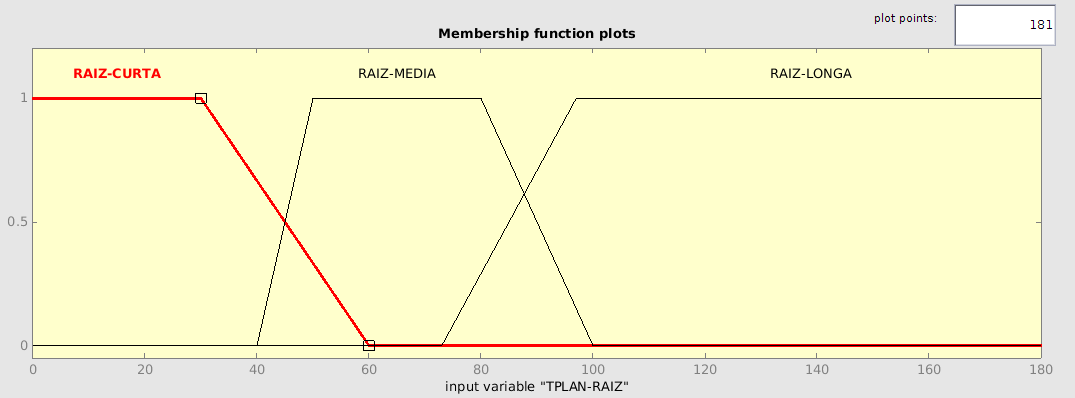
\includegraphics[width=1\linewidth]{Descricao/Imagens/TPLAN-RAIZ}
\caption{Tipo de raiz de cada planta}
\label{fig:TPLAN-RAIZ}
\end{figure}




